\chapter{Specifikacija programske potpore}
		
	\section{Funkcionalni zahtjevi}
			
			\noindent \textbf{Dionici:}
			
			\begin{packed_enum}
				
				\item Vlasnik (naručitelj)
				\item Stanovnik četvrti			
				\begin{packed_enum}
					\item  Obični stanovnik
					\item  Vijećnik
					\item  Moderator
				\end{packed_enum}
				\item Administrator	
				\item Razvojni tim
				
			\end{packed_enum}
			
			\noindent \textbf{Aktori i njihovi funkcionalni zahtjevi:}
			
			
			\begin{packed_enum}
			
				\item  \underbar{Neregistrirani korisnik (inicijator) može:}
				\begin{packed_enum}
					\item se registrirati u sustav stvaranjem novog korisničkog računa, za što su mu potrebni ime, prezime, adresa stanovanja, adresa e-pošte i lozinka
				\end{packed_enum}
				
				\item  \underbar{Neprijavljeni korisnik (inicijator) može:}
				\begin{packed_enum}
					\item se prijaviti u sustav,	za što su mu potrebni adresa e-pošte i lozinka
				\end{packed_enum}
				
				\item  \underbar{Stanovnik četvrti (inicijator) može:}
				\begin{packed_enum}
					\item čitati teme na "Forumu"
					\item otvarati teme na "Forumu"
					\item odgovarati u temama na "Forumu"
					\item uređivati svoje odgovore na "Forumu"
					\item ukloniti svoje odgovore na "Forumu"
					\item otvoriti temu na "Forumu" vezanu za objavu na "Vijeću četvrti", ako za tu objavu već nije otvorena tema
					\item čitati objave na "Vijeću četvrti"
					\item vidjeti najave događaja u cjelini "Događaji"
					\item predlagati najave budućih događaja u cjelini "Događaji", za što je potrebno navesti naziv, mjesto, vrijeme, trajanje i kratak opis
					\item poslati zahtjev administratorima za promjenu uloge (u "Vijećnika" ili "Moderatora")
					\item promijeniti osobne podatke	
					\item odjaviti se iz sustava
					\item obrisati svoj korisnički račun
				\end{packed_enum}
				
				\item  \underbar{Vijećnik (inicijator) može:}
				\begin{packed_enum}
					\item stvoriti objavu u cjelini "Vijeće četvrti"
					\item urediti objavu u cjelini "Vijeće četvrti"
					\item obrisati objavu u cjelini "Vijeće četvrti"	
				\end{packed_enum}
				
				\item  \underbar{Moderator (inicijator) može:}
				\begin{packed_enum}
					\item pregledati najave događaja koje predlažu stanovnici
					\item objaviti najave događaja u cjelini "Događaji"
					\item odbaciti prijedloge događaja
					\item urediti prijedloge događaja
					\item ukloniti odgovore u temama na "Forumu"
					\item ukloniti teme na Forumu
				\end{packed_enum}
				
				\item  \underbar{Administrator (inicijator) može:}
				\begin{packed_enum}
					\item vidjeti popis svih registriranih korisnika i njihove osobne podatke
					\item definirati četvrt i područje koje ta četvrt obuhvaća
					\item obrisati četvrti
					\item urediti podatke o četvrti
					\item vidjeti popis svih četvrti u sustavu
					\item odabrati pojedinu četvrt s popisa četvrti i pristupiti svom korisničkom sadržaju te četvrti
					\item pristupiti svim zahtjevima za uloge "Vijećnik" ili "Moderator"
					\item odbiti zahtjev za dodjelu uloge
					\item prihvatiti zahtjev za dodjelu uloge
					\item dodijeliti ulogu "Moderator" ili "Vijećnik" korisniku
					\item oduzeti ulogu "Moderator" ili "Vijećnik" korisniku
					\item privremeno blokirati korisnika
					\item pristupiti popisu blokiranih korisnika
					\item deblokirati korisnika
					\item trajno obrisati profil korisnika
				\end{packed_enum}
				
				\item  \underbar{Baza podataka (sudionik):}
				\begin{packed_enum}
					\item pohranjuje podatke o korisnicima i njihovim ovlastima
					\item pohranjuje podatke o četvrtima
					\begin{packed_enum}
						\item ulice koje im pripadaju
						\item teme na "Forumu"
						\item izvješća s "Vijeća četvrti"
						\item događaje iz sekcije "Događaji"
					\end{packed_enum}
				\end{packed_enum}
				
			\end{packed_enum}
			
			\eject 
			
			
				
			\subsection{Obrasci uporabe}
					
					\noindent \underbar{\textbf{UC1 - Registracija}}
					\begin{packed_item}
	
						\item \textbf{Glavni sudionik: }Korisnik
						\item  \textbf{Cilj:} Stvoriti korisnički račun
						\item  \textbf{Sudionici:} Baza podataka
						\item  \textbf{Preduvjet:} -
						\item  \textbf{Opis osnovnog tijeka:}
						
						\item[] \begin{packed_enum}
	
							\item Korisnik odabire opciju "Registracija"
							\item Korisnik unosi tražene podatke - ime, prezime, adresa stanovanja, adresa e-pošte i lozinka
							\item Korisnik odabire opciju "Podnesi"
							\item Korisnik dobiva obavijest o uspješnoj registraciji
							\item Korisnik biva preusmjeren na početnu stranicu
						\end{packed_enum}
						
						\item  \textbf{Opis mogućih odstupanja:}
						
						\item[] \begin{packed_item}
	
							\item[3.a] Korisnik odabire e-mail s kojim je već povezan korisnički račun u sustavu, ili unese tražene podatke u krivom formatu
							\item[] \begin{packed_enum}
								
								\item Korisnik dobiva obavijest o pogrešci
								\item Korisnik mijenja podatke i ponovno odabire opciju "Podnesi", ili odustaje od registracije
								
							\end{packed_enum}
							
						\end{packed_item}
					\end{packed_item}
					
					\noindent \underbar{\textbf{UC2 - Prijava}}
					\begin{packed_item}
	
						\item \textbf{Glavni sudionik: }Korisnik
						\item  \textbf{Cilj:} Dobiti pristup korisničkom dijelu sustava
						\item  \textbf{Sudionici:} Baza podataka
						\item  \textbf{Preduvjet:} -
						\item  \textbf{Opis osnovnog tijeka:}
						
						\item[] \begin{packed_enum}
	
							\item Korisnik odabire opciju "Prijava"
							\item Korisnik unosi e-mail adresu i lozinku
							\item Korisnik odabire opciju "Podnesi"
							\item Korisnik dobiva pristup korisničkom dijelu sustava
							\item Korisnik biva preusmjeren na početnu stranicu
						\end{packed_enum}
						
						\item  \textbf{Opis mogućih odstupanja:}
						
						\item[] \begin{packed_item}
	
							\item[3.a] Korisnik unosi e-mail s kojim nije povezan niti jedan korisnički račun, ili unosi krivu lozinku, ili unosi tražene podatke u krivom formatu
							\item[] \begin{packed_enum}
								
								\item Korisnik dobiva obavijest o pogrešci
								\item Korisnik mijenja podatke i ponovno odabire opciju "Podnesi", ili odustaje od prijave
								
							\end{packed_enum}
							
						\end{packed_item}
					\end{packed_item}
					
					
					\noindent \underbar{\textbf{UC3 - Odjava}}
					\begin{packed_item}
	
						\item \textbf{Glavni sudionik: }Korisnik
						\item  \textbf{Cilj:} Odjaviti se iz sustava
						\item  \textbf{Sudionici:} -
						\item  \textbf{Preduvjet:} Korisnik je prijavljen u sustav
						\item  \textbf{Opis osnovnog tijeka:}
						
						\item[] \begin{packed_enum}
	
							\item Korisnik odabire opciju "Odjava"
							\item Korisnik gubi pristup korisničkom dijelu sustava
							\item Korisnik biva preusmjeren na stranicu "Prijava"
						\end{packed_enum}
					\end{packed_item}					
					
					
					\noindent \underbar{\textbf{UC4 - Pregled osobnih podataka}}
					\begin{packed_item}
	
						\item \textbf{Glavni sudionik: }Korisnik
						\item  \textbf{Cilj:} Vidjeti osobne podatke
						\item  \textbf{Sudionici:} Baza podataka
						\item  \textbf{Preduvjet:} Korisnik je prijavljen u sustav
						\item  \textbf{Opis osnovnog tijeka:}
						
						\item[] \begin{packed_enum}
	
							\item Korisnik odabire opciju "Osobni podaci"
							\item Korisnik biva preusmjeren na stranicu "Osobni podaci" gdje dobije prikaz svojih osobnih podataka
						\end{packed_enum}
					\end{packed_item}
					
					\noindent \underbar{\textbf{UC5 - Promjena osobnih podataka}}
					\begin{packed_item}
	
						\item \textbf{Glavni sudionik: }Korisnik
						\item  \textbf{Cilj:} Promijeniti osobne podatke
						\item  \textbf{Sudionici:} Baza podataka
						\item  \textbf{Preduvjeti:}
						\item[] \begin{packed_enum}
							\item Korisnik je prijavljen u sustav
							\item Korisnik pregledava svoje osobne podatke (UC4)
						\end{packed_enum}
						\item  \textbf{Opis osnovnog tijeka:}
						
						\item[] \begin{packed_enum}
	
							\item Korisnik odabire opciju "Promjena osobnih podataka"
							\item Korisnik mijenja svoje podatke
							\item Korisnik odabire opciju "Spremi promjene"
							\item Baza podataka se ažurira
							\item Korisnik biva preusmjeren na stranicu "Osobni podaci"
						\end{packed_enum}
						
						\item  \textbf{Opis mogućih odstupanja:}
						
						\item[] \begin{packed_item}
	
							\item[3.a] Korisnik mijenja svoje osobne podatke, ali ne spremi promjene
							\item[] \begin{packed_enum}
								
								\item Sustav upozori korisnika da nije spremio promjene
								\item Korisnik spremi promjene, ili odustane od njih
								
							\end{packed_enum}
							
							\item[3.b] Korisnik pokuša promijeniti e-mail adresu
							\item[] \begin{packed_enum}
								
								\item Sustav upozori korisnika da ne može promijeniti e-mail adresu
								\item Korisnik promijeni neke druge osobne podatke, ili odustane od promjena
								
							\end{packed_enum}
							
							\item[3.c] Korisnik pokuša promijeniti neki osobni podatak u nedozvoljeni format (npr. ime koje počinje malim slovom), ili pokuša promijeniti adresu na neku adresu koja ne postoji u sustavu
							\item[] \begin{packed_enum}
								
								\item Sustav upozori korisnika o pogrešci
								\item Korisnik pokuša promijeniti svoje osobne podatke u ispravan format, ili odustane od promjena
								
							\end{packed_enum}
							
							\item[3.d] Korisnik je promijenio adresu, i nova adresa ne pripada kvartu kojem je pripadala njegova stara adresa
							\item[] \begin{packed_enum}
								
								\item Sustav dodijeli korisnika novom kvartu
								\item Sustav korisniku oduzima uloge "Vijećnik" i "Moderator", ako ih ima
								\item Baza podataka se ažurira
								\item Korisnik biva preusmjeren na stranicu "Osobni podaci"
								
							\end{packed_enum}
							
						\end{packed_item}
					\end{packed_item}
					
					\noindent \underbar{\textbf{UC6 - Brisanje korisničkog računa}}
					\begin{packed_item}
	
						\item \textbf{Glavni sudionik: }Korisnik
						\item  \textbf{Cilj:} Obrisati korisnički račun
						\item  \textbf{Sudionici:} Baza podataka
						\item  \textbf{Preduvjeti:}
						\item[] \begin{packed_enum}
							\item Korisnik je prijavljen u sustav
							\item Korisnik pregledava svoje osobne podatke (UC4)
							\item Korisnik nema ulogu "Administrator"
						\end{packed_enum}
						\item  \textbf{Opis osnovnog tijeka:}
						
						\item[] \begin{packed_enum}
	
							\item Korisnik odabire opciju "Obriši korisnički račun"
							\item Sustav upozori korisnika da je brisanje korisničkog računa trajna i nepovratna akcija
							\item Korisnik potvrđuje svoj odabir
							\item Korisnički račun se izbriše iz baze podataka
							\item Korisnik biva preusmjeren na stranicu "Prijava"
							
						\end{packed_enum}
						
						\item  \textbf{Opis mogućih odstupanja:}
						
						\item[] \begin{packed_item}
	
							\item[3.a] Korisnik odustane od brisanja svog računa
							\item[] \begin{packed_enum}
								
								\item Korisnik biva preusmjeren na stranicu "Osobni podaci"
														
							\end{packed_enum}
							
						\end{packed_item}
					\end{packed_item}
					
					
					\noindent \underbar{\textbf{UC7 - Promjena adrese radi ispravljanja nevažećeg statusa stanovanja}}
                    \begin{packed_item}
    
                        \item \textbf{Glavni sudionik: }Korisnik
                        \item  \textbf{Cilj:} Promijeniti adresu i omogućiti korisniku pristup korisničkom dijelu sustava
                        \item  \textbf{Sudionici:} Baza podataka
                        \item  \textbf{Preduvjeti:}
						\item[] \begin{packed_enum}
							\item Korisnik je prijavljen u sustav
							\item Korisnikov status stanovanja je "Nevažeći"
						\end{packed_enum}
                        \item  \textbf{Opis osnovnog tijeka:}
                        
                        \item[] \begin{packed_enum}
    
                            \item Korisnik ispunjava obrazac u kojem unosi novu adresu
                            \item Korisnik odabire opciju "Spremi promjene"
                            \item Baza podataka se ažurira
                            \item Korisnik biva preusmjeren na početnu stranicu
                        \end{packed_enum}
                        
                        \item  \textbf{Opis mogućih odstupanja:}
                        
                        \item[] \begin{packed_item}
    
                            \item[2.a] Korisnik nije unio novu adresu, ili je adresa koju je korisnik unio nevažeća
                            \item[] \begin{packed_enum}
                                
                                \item Sustav upozorava korisnika o pogrešci
                                \item Korisnik ispravlja pogrešku i ponovno odabire opciju "Spremi promjene", ili odustaje od ispravljanja adrese
                                
                            \end{packed_enum}
                            
                        \end{packed_item}
                    \end{packed_item}					
					

					\noindent \underbar{\textbf{UC8 - Pregled događaja u cjelini "Događaji" }}
					\begin{packed_item}
	
						\item \textbf{Glavni sudionik: }Korisnik
						\item  \textbf{Cilj:} Prikaz potvrđenih događaja u korisnikovom kvartu
						\item  \textbf{Sudionici:} Baza podataka
						\item  \textbf{Preduvjet:} Korisnik je prijavljen u sustav
						\item  \textbf{Opis osnovnog tijeka:}
						
						\item[] \begin{packed_enum}
	
							\item Korisnik odabere opciju "Događaji"
							\item Korisnik biva preusmjeren na stranicu "Događaji" gdje dobije prikaz potvrđenih događaja u njegovom kvartu
						\end{packed_enum}
						
							
						\end{packed_item}
					\noindent \underbar{\textbf{UC9 - Stvaranje prijedloga događaja}}
					\begin{packed_item}
	
						\item \textbf{Glavni sudionik: }Korisnik
						\item  \textbf{Cilj:} Stvoriti prijedlog događaja
						\item  \textbf{Sudionici:} Baza podataka
						\item  \textbf{Preduvjeti:}
						\item[] \begin{packed_enum}
							\item Korisnik je prijavljen u sustav
							\item Korisnik pregledava događaje (UC8)
						\end{packed_enum}
						\item  \textbf{Opis osnovnog tijeka:}
						
						\item[] \begin{packed_enum}
	
							\item Korisnik odabire opciju "Novi prijedlog događaja" 
							\item Korisnik ispunjava polja "naziv", "mjesto", "vrijeme", "trajanje" i "kratki opis"
							\item Korisnik odabire opciju "Objavi prijedlog događaja"
							\item Baza podataka se ažurira
						\end{packed_enum}
						
						\item  \textbf{Opis mogućih odstupanja:}
						
						\item[] \begin{packed_item}
	
							\item[3.a] Korisnik nije ispunio sva polja prilikom stvaranja prijedloga događaja
							\item[] \begin{packed_enum}
								
								\item Sustav upozori korisnika da sva polja nisu ispunjena
								\item Korisnik ispuni preostala polja i odabire opciju "Objavi prijedlog događaja", ili odustane od prijedloga
							\end{packed_enum}
								
							\item[3.b] Korisnik pokuša napustiti stranicu prije biranja opcije "Objavi prijedlog događaja"
							\item[] \begin{packed_enum}
								
								\item Sustav upozori korisnika da se skica prijedloga događaja neće spremiti
								\item Korisnik odabire opciju "Objavi prijedlog događaja", ili odustaje od objave prijedloga događaja
								
							\end{packed_enum}
							
							
						\end{packed_item}
					\end{packed_item}						
					\noindent \underbar{\textbf{UC10 - Pregled prijedloga događaja}}
					\begin{packed_item}
	
						\item \textbf{Glavni sudionik: }Moderator
						\item  \textbf{Cilj:} Pregled prijedloga događaja u cjelini "Događaji"
						\item  \textbf{Sudionici:} Baza podataka
						\item  \textbf{Preduvjeti:}
						\item[] \begin{packed_enum}
							\item Korisnik je prijavljen u sustav
							\item Korisnik ima ulogu "Moderator"
							\item Korisnik pregledava događaje (UC8)
						\end{packed_enum}
						\item  \textbf{Opis osnovnog tijeka:}
						
						\item[] \begin{packed_enum}
	
							\item Korisnik odabire opciju "Prijedlozi događaja" 
							\item Korisnik biva preusmjeren na stranicu "Prijedlozi događaja" gdje dobije prikaz svih prijedloga događaja za svoj kvart
							
						\end{packed_enum}
						\end{packed_item}
						
						\eject
						
						\noindent \underbar{\textbf{UC11 - Uređivanje prijedloga događaja}}
					\begin{packed_item}
	
						\item \textbf{Glavni sudionik: }Moderator
						\item  \textbf{Cilj:} Uređivanje prijedloga događaja u cjelini "Događaji"
						\item  \textbf{Sudionici:} Baza podataka
						\item  \textbf{Preduvjeti:}
						\item[] \begin{packed_enum}
							\item Korisnik je prijavljen u sustav
							\item Korisnik ima ulogu "Moderator"
							\item Korisnik pregledava prijedloge događaja (UC10)
						\end{packed_enum}
						\item  \textbf{Opis osnovnog tijeka:}
						
						\item[] \begin{packed_enum}
	
							\item Korisnik odabire prijedlog događaja 
							\item Korisnik odabire opciju "Uredi prijedlog događaja"
							\item Korisnik uređuje polja za odabrani prijedlog događaja
							\item Korisnik odabire opciju "Spremi promjene"
							\item Baza podataka se ažurira
							
						\end{packed_enum}
						\item  \textbf{Opis mogućih odstupanja:}
						
						\item[] \begin{packed_item}
	
							\item[4.a] Korisnik nije spremio promjene
							\item[] \begin{packed_enum}
								
								\item Sustav upozori korisnika da promjene nisu spremljene
								\item Korisnik odabire opciju "Spremi promjene", ili odustane od promjena
								
							\end{packed_enum}
							
							\item[4.b] Korisnik obriše neko polje, tj. ostavi ga praznim nakon unošenja promjena
							\item[] \begin{packed_enum}
								
								\item Sustav upozori korisnika da niti jedno polje u formularu ne može biti prazno
								\item Korisnik ispuni to polje i odabire opciju "Spremi promjene", ili odustane od promjena
								
							\end{packed_enum}
							
							
						\end{packed_item}
						\end{packed_item}
					\noindent \underbar{\textbf{UC12 - Objava prijedloga događaja}}
					\begin{packed_item}
	
						\item \textbf{Glavni sudionik: }Moderator
						\item  \textbf{Cilj:} Objava predloženog događaja u cjelini "Događaji"
						\item  \textbf{Sudionici:} Baza podataka
						\item  \textbf{Preduvjeti:}
						\item[] \begin{packed_enum}
							\item Korisnik je prijavljen u sustav
							\item Korisnik ima ulogu "Moderator"
							\item Korisnik pregledava prijedloge događaja (UC10)
						\end{packed_enum}
						\item  \textbf{Opis osnovnog tijeka:}
						
						\item[] \begin{packed_enum}
	
							\item Korisnik odabire prijedlog događaja 
							\item Korisnik odabire opciju "Objavi događaj"
							\item Baza podataka se ažurira
							
						\end{packed_enum}
						\end{packed_item}
					\noindent \underbar{\textbf{UC13 - Brisanje prijedloga događaja}}
					\begin{packed_item}
	
						\item \textbf{Glavni sudionik: }Moderator
						\item  \textbf{Cilj:} Brisanje prijedloga događaja u cjelini "Događaji"
						\item  \textbf{Sudionici:} Baza podataka
						\item  \textbf{Preduvjeti:}
						\item[] \begin{packed_enum}
							\item Korisnik je prijavljen u sustav
							\item Korisnik ima ulogu "Moderator"
							\item Korisnik pregledava prijedloge događaja (UC10)
						\end{packed_enum}
						\item  \textbf{Opis osnovnog tijeka:}
						
						\item[] \begin{packed_enum}
	
							\item Korisnik odabire prijedlog događaja 
							\item Korisnik odabire opciju "Obriši prijedlog događaja"
							\item Baza podataka se ažurira
							
						\end{packed_enum}
						
					\end{packed_item}
					\noindent \underbar{\textbf{UC14 - Pregled tema na "Forumu"}}
					\begin{packed_item}
	
						\item \textbf{Glavni sudionik: }Korisnik
						\item  \textbf{Cilj:} Prikaz tema na "Forumu"
						\item  \textbf{Sudionici:} Baza podataka
						\item  \textbf{Preduvjet:} Korisnik je prijavljen u sustav
						\item  \textbf{Opis osnovnog tijeka:}
						
						\item[] \begin{packed_enum}
	
							\item Korisnik odabire cjelinu "Forum"
							\item Korisnik biva preusmjeren na stranicu "Forum" gdje gdje dobije prikaz tema na "Forumu", poredanih po vremenu zadnjeg odgovora
							
						\end{packed_enum}
						
						
					\end{packed_item}						
					\noindent \underbar{\textbf{UC15 - Prikaz teme na "Forumu"}}
					\begin{packed_item}
	
						\item \textbf{Glavni sudionik: }Korisnik
						\item  \textbf{Cilj:} Odabrati temu na "Forumu" i vidjeti sve objave u njoj
						\item  \textbf{Sudionici:} Baza podataka
						\item  \textbf{Preduvjeti:}
						\item[] \begin{packed_enum}
							\item Korisnik je prijavljen u sustav
							\item Korisnik pregledava "Forum" (UC14)
						\end{packed_enum}
						\item  \textbf{Opis osnovnog tijeka:}
						
						\item[] \begin{packed_enum}
	
							\item Korisnik u cjelini "Forum" odabire željenu temu
							\item Prikazuje se odabrana tema
							
						\end{packed_enum}
						
					\end{packed_item}
					
					
					\noindent \underbar{\textbf{UC16 - Otvaranje teme na "Forumu"}}
                    \begin{packed_item}
    
                        \item \textbf{Glavni sudionik: }Korisnik
                        \item  \textbf{Cilj:} Otvoriti temu na "Forumu"
                        \item  \textbf{Sudionici:} Baza podataka
                        \item  \textbf{Preduvjeti:}
						\item[] \begin{packed_enum}
							\item Korisnik je prijavljen u sustav
							\item Korisnik pregledava "Forum" (UC14)
						\end{packed_enum}
                        \item  \textbf{Opis osnovnog tijeka:}
                        
                        \item[] \begin{packed_enum}
    
                            \item Korisnik odabire opciju "Otvori novu temu"
                            \item Korisnik ispunjava obrazac s imenom novootvorene teme i prvom objavom u toj temi
                            \item Korisnik odabire opciju "Otvori temu"
                            \item Baza podataka se ažurira
                            \item Korisnik biva preusmjeren na stranicu koja odgovara novootvorenoj temi
                        \end{packed_enum}
                        
                        \item  \textbf{Opis mogućih odstupanja:}
						
						\item[] \begin{packed_item}
						\item[3.a] Korisnik nije ispunio sva polja u obrascu s imenom i prvom objavom u temi
							\item[] \begin{packed_enum}
								
								\item Sustav upozorava korisnika da mora ispuniti sva polja u obrascu
								\item Korisnik ispunjava polja i ponovno odabire opciju "Otvori temu", ili odustaje od otvaranja teme
								
							\end{packed_enum}
                    		\end{packed_item}	
                    	\end{packed_item}				
					
					\noindent \underbar{\textbf{UC17 - Odgovaranje na objavu u temi na "Forumu"}}
					\begin{packed_item}
	
						\item \textbf{Glavni sudionik: }Korisnik
						\item  \textbf{Cilj:} Odgovoriti na željenu objavu u temi na "Forumu"
						\item  \textbf{Sudionici:} Baza podataka
						\item  \textbf{Preduvjeti:}
						\item[] \begin{packed_enum}
							\item Korisnik je prijavljen u sustav
							\item Korisnik pregledava temu na "Forumu" (UC15)
						\end{packed_enum}
						\item  \textbf{Opis osnovnog tijeka:}
						
						\item[] \begin{packed_enum}
	
							\item Korisnik unutar teme na "Forumu" na odabranoj objavi odabire opciju "Odgovori"
							\item Otvara se polje za odgovor
							\item Korisnik ispunjava polje za odgovor tekstom
							\item Korisnik bira opciju "Objavi odgovor"
							\item Baza podataka se ažurira
							\item Korisnik biva preusmjeren na stranicu koja odgovara toj temi na "Forumu"
							
							
						\end{packed_enum}
						
						\item  \textbf{Opis mogućih odstupanja:}
						
						\item[] \begin{packed_item}
						\item[3.a] Korisnik pokuša objaviti odgovor bez teksta
							\item[] \begin{packed_enum}
								
								\item Sustav upozorava korisnika da odgovor na "Forumu" ne može biti prazan tekst
								\item Korisnik doda tekst u polje za tekst odgovora, ili odustane od objave odgovora
								
							\end{packed_enum}
						
						
					\end{packed_item}
					\end{packed_item}
					\noindent \underbar{\textbf{UC18 - Uređivanje odgovora u temi na "Forumu"}}
					\begin{packed_item}
	
						\item \textbf{Glavni sudionik: }Korisnik
						\item  \textbf{Cilj:} Uređivanje odgovora u temi na "Forumu" 
						\item  \textbf{Sudionici:} Baza podataka
						\item  \textbf{Preduvjeti:}
						\item[] \begin{packed_enum}
							\item Korisnik je prijavljen u sustav
							\item Korisnik pregledava temu na "Forumu" (UC15)
							\item Korisnik je autor odgovora kojeg odabire
						\end{packed_enum}
						\item  \textbf{Opis osnovnog tijeka:}
						
						\item[] \begin{packed_enum}
	
							\item Korisnik odabire opciju "Uredi odgovor"
							\item Otvara se polje za odgovor koje sadrži trenutnu verziju teksta odgovora
							\item Korisnik uređuje tekst
							\item Korisnik odabire opciju "Spremi promjene"
							\item Baza podataka se ažurira
							\item Korisnik biva preusmjeren na stranicu koja odgovara toj temi na "Forumu"
							
						\end{packed_enum}
							
						\item  \textbf{Opis mogućih odstupanja:}
						
						\item[] \begin{packed_item}
						\item[4.a] Korisnik napušta stranicu iako uređeni odgovor nije objavio
							\item[] \begin{packed_enum}
								
								\item Sustav upozorava korisnika da uređeni tekst neće biti spremljen ako napusti stranicu
								\item Korisnik odabire opciju "Spremi promjene", ili odustane od promjena
								
							\end{packed_enum}
						\item[4.b] Korisnik je obrisao sav tekst odgovora i odabrao opciju "Spremi promjene"
							\item[] \begin{packed_enum}
								
								\item Sustav upozorava korisnika da tekst objave ne smije biti prazan
								\item Korisnik u polje za tekst odgovora doda neki tekst, ili odustane od promjene odgovora
								
							\end{packed_enum}
						\end{packed_item}
						
					\end{packed_item}	
					
					\noindent \underbar{\textbf{UC19 - Brisanje odgovora u temi na "Forumu"}}
					\begin{packed_item}
	
						\item \textbf{Glavni sudionik: }Korisnik
						\item  \textbf{Cilj:} Obrisati odgovor u temi na "Forumu"
						\item  \textbf{Sudionici:} Baza podataka
						\item  \textbf{Preduvjeti:}
						\item[] \begin{packed_enum}
							\item Korisnik je prijavljen u sustav
							\item Korisnik pregledava temu na "Forumu" (UC15)
							\item Korisnik odabire odgovor čiji autor je on, ili korisnik ima ulogu "Moderator"
						\end{packed_enum}
						\item  \textbf{Opis osnovnog tijeka:}
						
						\item[] \begin{packed_enum}
	
							\item Korisnik pronalazi odgovor koji želi obrisati
							\item Korisnik odabire opciju "Izbriši odgovor"
							\item Sustav upozorava korisnika da je brisanje odgovora trajna i nepovratna akcija
							\item Korisnik potvrđuje svoj odabir
							\item Baza podataka se ažurira
							\item Korisnik biva preusmjeren na stranicu koja odgovara toj temi na "Forumu"
							
							
						\end{packed_enum}
						
						\item  \textbf{Opis mogućih odstupanja:}
						
						\item[] \begin{packed_item}
						\item[4.a] Korisnik odustane od brisanja odgovora
							\item[] \begin{packed_enum}
								
								\item Prozor za brisanje odgovora se ugasi
								
							\end{packed_enum}
						\item[4.b] Korisnik je obrisao posljednji odgovor u odgovarajućoj temi
							\item[] \begin{packed_enum}
								
								\item Sustav automatski obriše tu temu na "Forumu"
								\item Baza podataka se ažurira
								\item Korisnik biva preusmjeren na stranicu "Forum"
								
							\end{packed_enum}
						\end{packed_item}
						
						
					\end{packed_item}
					
					\noindent \underbar{\textbf{UC20 - Brisanje teme na "Forumu"}}
					\begin{packed_item}
	
						\item \textbf{Glavni sudionik: }Moderator
						\item  \textbf{Cilj:} Obrisati temu na "Forumu"
						\item  \textbf{Sudionici:} Baza podataka
						\item  \textbf{Preduvjeti:}
						\item[] \begin{packed_enum}
							\item Korisnik je prijavljen u sustav
							\item Korisnik pregledava "Forum" (UC14)
							\item Korisnik ima ulogu "Moderator"
						\end{packed_enum}
						\item  \textbf{Opis osnovnog tijeka:}
						
						\item[] \begin{packed_enum}
	
							\item Korisnik odabire opciju "Obriši temu"
							\item Sustav upozorava korisnika da je brisanje teme trajna i nepovratna akcija
							\item Korisnik potvrđuje svoju odluku i tema se obriše
							\item Baza podataka se ažurira
							\item Korisnik biva preusmjeren na stranicu "Forum"
						\end{packed_enum}
						
						\item  \textbf{Opis mogućih odstupanja:}
						
						\item[] \begin{packed_item}
	
							\item[3.a] Korisnik odustane od brisanja teme
							\item[] \begin{packed_enum}
								
								\item Korisnik biva preusmjeren na stranicu "Forum"
								
							\end{packed_enum}
							
						\end{packed_item}
					\end{packed_item}					
										
					\noindent \underbar{\textbf{UC21 - Pregled cjeline "Vijeće četvrti" }}
					\begin{packed_item}
	
						\item \textbf{Glavni sudionik: }Korisnik
						\item  \textbf{Cilj:} Pregled svih izvješća u cjelini "Vijeće četvrti"
						\item  \textbf{Sudionici:} Baza podataka
						\item  \textbf{Preduvjet:} Korisnik je prijavljen u sustav
						\item  \textbf{Opis osnovnog tijeka:}
						
						\item[] \begin{packed_enum}
	
							\item Korisnik odabire opciju "Vijeće četvrti" 
							\item Korisnik biva preusmjeren na stranicu "Vijeće četvrti" gdje dobije prikaz svih izvješća, poredanih kronološki od najsvježijeg
							
							
						\end{packed_enum}

						
					\end{packed_item}		
					
					\noindent \underbar{\textbf{UC22 - Prikaz izvješća u "Vijeću četvrti" }}
					\begin{packed_item}
	
						\item \textbf{Glavni sudionik: }Korisnik
						\item  \textbf{Cilj:} Prikaz jednog izvješća u cjelini "Vijeće četvrti"
						\item  \textbf{Sudionici:} Baza podataka
						\item  \textbf{Preduvjeti:}
						\item[] \begin{packed_enum}
							\item Korisnik je prijavljen u sustav
							\item Korisnik pregledava "Vijeće četvrti" (UC21)
						\end{packed_enum}
						\item  \textbf{Opis osnovnog tijeka:}
						
						\item[] \begin{packed_enum}
	
							\item Korisnik odabire izvješće koje želi pregledati 
							\item Korisnik biva preusmjeren na stranicu koja odgovara izvješću koje je odabrao
							
							
						\end{packed_enum}

						
					\end{packed_item}							
								
					\noindent \underbar{\textbf{UC23 - Objava novog izvješća na "Vijeću četvrti"}}
					\begin{packed_item}
	
						\item \textbf{Glavni sudionik: }Vijećnik
						\item  \textbf{Cilj:} Objaviti novo izvješće na "Vijeću četvrti"
						\item  \textbf{Sudionici:} Baza podataka
						\item  \textbf{Preduvjeti:}
						\item[] \begin{packed_enum}
							\item Korisnik je prijavljen u sustav
							\item Korisnik pregledava "Vijeće četvrti" (UC21)
							\item Korisnik ima ulogu "Vijećnik"
						\end{packed_enum}
						\item  \textbf{Opis osnovnog tijeka:}
						
						\item[] \begin{packed_enum}
	
							\item Korisnik odabire opciju "Stvaranje novog izvješća" 
							\item Otvara se polje za pisanje izvješća
							\item Korisnik ispunjava polje tekstom izvješća
							\item Korisnik odabire opciju "Objavi izvješće"
							\item Baza podataka se ažurira
							\item Korisnik biva preusmjeren na stranicu "Vijeća četvrti"
							
							
						\end{packed_enum}
						
						\item  \textbf{Opis mogućih odstupanja:}
						
						\item[] \begin{packed_item}
	
							\item[4.a] Korisnik pokuša objaviti prazno izvješće bez teksta
							\item[] \begin{packed_enum}
								
								\item Sustav upozorava korisnika da izvješće s "Vijeća četvrti" ne može biti prazan tekst
								\item Korisnik doda tekst u polje za tekst izvješća, ili odustane od objave izvješća
							\end{packed_enum}
								
							\item[4.b] Korisnik pokuša napustiti stranicu bez biranja opcije "Objavi izvješće"
							\item[] \begin{packed_enum}
								
								\item Sustav upozorava korisnika da skica izvješća neće biti objavljena
								\item Korisnik odabire opciju "Objavi izvješće", ili odustaje od objave
								
							\end{packed_enum}
							
						\end{packed_item}
						
						
					\end{packed_item}					
					\noindent \underbar{\textbf{UC24 - Uređivanje izvješća na "Vijeću četvrti"}}
					\begin{packed_item}
	
						\item \textbf{Glavni sudionik: }Vijećnik
						\item  \textbf{Cilj:} Urediti izvješće
						\item  \textbf{Sudionici:} Baza podataka
						\item  \textbf{Preduvjeti:}
						\item[] \begin{packed_enum}
							\item Korisnik je prijavljen u sustav
							\item Korisnik pregledava izvješće s "Vijeća četvrti" (UC22)
							\item Korisnik ima ulogu "Vijećnik"
							\item Korisnik je autor izvješća kojeg pregledava
						\end{packed_enum}
						\item  \textbf{Opis osnovnog tijeka:}
						
						\item[] \begin{packed_enum}
	
							\item Korisnik odabire opciju "Uredi izvješće"
							\item Otvara se tekstualno polje koje sadrži trenutnu verziju izvješća
							\item Korisnik uređuje tekst
							\item Korisnik odabire opciju "Spremi promjene"
							\item Baza podataka se ažurira
							\item Korisnik biva preusmjeren na stranicu koja odgovara tom izvješću na "Vijeću četvrti"
							
							
							
						\end{packed_enum}
						\item  \textbf{Opis mogućih odstupanja:}
						
						\item[] \begin{packed_item}
						\item[4.a] Korisnik napušta stranicu iako uređeno izvješće nije objavio
							\item[] \begin{packed_enum}
								
								\item Sustav upozorava korisnika da uređeni tekst neće biti spremljen ako napusti stranicu
								\item Korisnik odabire opciju "Spremi promjene", ili odustane od promjena
								
							\end{packed_enum}
							
						\item[4.b] Korisnik je obrisao sav tekst izvješća i odabrao opciju "Spremi promjene"
							\item[] \begin{packed_enum}
								
								\item Sustav upozorava korisnika da tekst izvješća ne smije biti prazan
								\item Korisnik u polje za tekst izvješća doda neki tekst, ili odustane od promjene izvješća
								
							\end{packed_enum}
						\end{packed_item}
						
						
						
					\end{packed_item}					
					

					\noindent \underbar{\textbf{UC25 - Brisanje izvješća na "Vijeću četvrti"}}
					\begin{packed_item}
	
						\item \textbf{Glavni sudionik: }Vijećnik
						\item  \textbf{Cilj:} Obrisati izvješće u cjelini "Vijeće četvrti"
						\item  \textbf{Sudionici:} Baza podataka
						\item  \textbf{Preduvjeti:}
						\item[] \begin{packed_enum}
							\item Korisnik je prijavljen u sustav
							\item Korisnik pregledava izvješće s "Vijeća četvrti" (UC22)
							\item Korisnik ima ulogu "Vijećnik"														\end{packed_enum}
						\item  \textbf{Opis osnovnog tijeka:}
						
						\item[] \begin{packed_enum}
	
							\item Korisnik odabire opciju "Obriši izvješće"
							\item Sustav upozorava korisnika da je brisanje izvješća trajna i nepovratna akcija
							\item Korisnik potvrđuje svoju odluku i izvješće se obriše
							\item Baza podataka se ažurira
							\item Korisnik biva preusmjeren na stranicu "Vijeće četvrti"
						\end{packed_enum}
						
						\item  \textbf{Opis mogućih odstupanja:}
						
						\item[] \begin{packed_item}
	
							\item[3.a] Korisnik odustane od brisanja izvješća
							\item[] \begin{packed_enum}
								
								\item Korisnik biva preusmjeren na stranicu koja odgovara tom izvješću
								
							\end{packed_enum}
							
						\end{packed_item}
					\end{packed_item}
						
						
						
					\noindent \underbar{\textbf{UC26 - Otvaranje teme na "Forumu" vezanu za izvješće s "Vijeća četvrti"}}
					\begin{packed_item}
	
						\item \textbf{Glavni sudionik: }Korisnik
						\item  \textbf{Cilj:} Na "Forumu" stvoriti temu vezanu uz izvješće na "Vijeću četvrti"
						\item  \textbf{Sudionici:} Baza podataka
						\item  \textbf{Preduvjeti:}
						\item[] \begin{packed_enum}
							\item Korisnik je prijavljen u sustav
							\item Korisnik pregledava izvješće s "Vijeća četvrti" (UC22)
							\item Za odabrano izvješće nije već otvorena tema na "Forumu"								\end{packed_enum}
						\item  \textbf{Opis osnovnog tijeka:}
						
						\item[] \begin{packed_enum}
	
							\item Korisnik odabire opciju "Otvori temu na 'Forumu'"
							\item Korisnik ispunjava obrazac s prvom objavom u novootvorenoj temi, za ime teme se automatski postavlja naslov izvješća, a kao nulta objava u novootvorenoj temi se postavlja tekst izvješća s autorom "Vijeće četvrti"
							\item Korisnik odabire opciju "Otvori temu"
							\item Otvara se nova tema na cjelini "Forum"
							\item Baza podataka se ažurira
							\item Korisnik biva preusmjeren na novootvorenu temu na "Forumu"
							
						\end{packed_enum}	
						
						\item  \textbf{Opis mogućih odstupanja:}
						
						\item[] \begin{packed_item}
						\item[3.a] Korisnik nije ispunio obrazac s prvom objavom u temi
							\item[] \begin{packed_enum}
								
								\item Sustav upozorava korisnika da mora ispuniti sva polja u obrascu
								\item Korisnik ispunjava polja i ponovno odabire opciju "Otvori temu", ili odustaje od otvaranja teme
								
							\end{packed_enum}
                    		\end{packed_item}				
						
					\end{packed_item}
					
					\noindent \underbar{\textbf{UC27 - Podnošenje zahtjeva za dodjelu uloge}}
					\begin{packed_item}
	
						\item \textbf{Glavni sudionik: }Korisnik
						\item  \textbf{Cilj:} Priložiti zahtjev za promjenu uloge
						\item  \textbf{Sudionici:} Baza podataka
						\item  \textbf{Preduvjeti:}
						\item[] \begin{packed_enum}
							\item Korisnik je prijavljen u sustav
							\item Korisnik nema ulogu za koju šalje zahtjev
							\item Korisnik pregledava svoje osobne podatke (UC4)
							\item Korisnik već nije predao zahtjev za ulogom koju sad traži čiji je status trenutno "Nerazriješen"
							\item Korisnik nema ulogu "Administrator"
							\end{packed_enum}
						\item  \textbf{Opis osnovnog tijeka:}
						
						\item[] \begin{packed_enum}
	
							\item Korisnik odabire opciju "Novi zahtjev za ulogom"
							\item Korisnik odabire ulogu za koju šalje zahtjev
							\item Korisnik pošalje zahtjev
							\item Baza podataka se ažurira
						\end{packed_enum}
						
						\item  \textbf{Opis mogućih odstupanja:}
						
						\item[] \begin{packed_item}
						
							\item[3.a] Korisnik pokuša poslati zahtjev bez da je odabrao ulogu
							\item[] \begin{packed_enum}
								
								\item Sustav upozori korisnika da nije odabrao ulogu
								\item Korisnik odabere ulogu, ili odustane od zahtjeva
								
							\end{packed_enum}
	
							\item[3.b] Korisnik pokuša ugasiti prozor za zahtjev za ulogu bez da je poslao zahtjev
							\item[] \begin{packed_enum}
								
								\item Sustav upozori korisnika da nije poslao zahtjev
								\item Korisnik pošalje zahtjev, ili odustane od njega
								
							\end{packed_enum}
							
						\end{packed_item}
					\end{packed_item}
					
					\noindent \underbar{\textbf{UC28 - Pregled svih korisnika u sustavu}}
					\begin{packed_item}
	
						\item \textbf{Glavni sudionik: }Administrator
						\item  \textbf{Cilj:} Pristupiti popisu svih korisnika u sustavu
						\item  \textbf{Sudionici:} Baza podataka
						\item  \textbf{Preduvjeti:}
						\item[] \begin{packed_enum}
							\item Korisnik je prijavljen u sustav
							\item Korisnik ima ulogu "Administrator"
							\end{packed_enum}
						\item  \textbf{Opis osnovnog tijeka:}
						
						\item[] \begin{packed_enum}
	
							\item Korisnik odabire opciju "Korisnici"
							\item Korisnik biva preusmjeren na stranicu "Korisnici" gdje dobije popis svih korisnika sustava
						\end{packed_enum}
					
					\end{packed_item}
					
					\noindent \underbar{\textbf{UC29 - Pregled korisnika}}
					\begin{packed_item}
	
						\item \textbf{Glavni sudionik: } Administrator
						\item  \textbf{Cilj:} Pregledati osobne podatke korisnika (radi jednoznačnosti, u daljnjem tekstu: objekt)
						\item  \textbf{Sudionici:} Baza podataka
						\item  \textbf{Preduvjeti:}
						\item[] \begin{packed_enum}
							\item Korisnik je prijavljen u sustav
							\item Korisnik ima ulogu "Administrator"
							\item Korisnik pregledava sve korisnike u sustavu (UC28)
						\end{packed_enum}
						\item  \textbf{Opis osnovnog tijeka:}
						
						\item[] \begin{packed_enum}
	
							\item Korisnik odabire objekta čije osobne podatke želi pregledati
							\item Korisnik biva preusmjeren na stranicu s osobnim podacima objekta
						\end{packed_enum}
						
					\end{packed_item}
					
					\noindent \underbar{\textbf{UC30 - Dodjela uloge}}
					\begin{packed_item}
	
						\item \textbf{Glavni sudionik: }Administrator
						\item  \textbf{Cilj:} Dodijeliti ulogu korisniku (radi jednoznačnosti, u daljnjem tekstu: objekt)
						\item  \textbf{Sudionici:} Baza podataka
						\item  \textbf{Preduvjeti:}
						\item[] \begin{packed_enum}
							\item Korisnik je prijavljen u sustav
							\item Korisnik ima ulogu "Administrator"
							\item Korisnik pregledava osobne podatke objekta (UC29)
							\item Objekt nema ulogu koju mu korisnik želi dodijeliti
							\item Objekt nema ulogu "Administrator"
						\end{packed_enum}
						\item  \textbf{Opis osnovnog tijeka:}
						
						\item[] \begin{packed_enum}
	
							\item Korisnik odabire ulogu koju želi dodijeliti objektu
							\item Baza podataka se ažurira
							\item Korisnik biva preusmjeren na stranicu s osobnim podacima objekta
						\end{packed_enum}
						
						\item  \textbf{Opis mogućih odstupanja:}
						
						\item[] \begin{packed_item}
						\item[1.a] Postoji zahtjev za ulogom sa statusom "Nerazriješen" čiji je autor objekt i kojem je uloga jednaka ulozi koji je korisnik manualno dodijelio objektu
							\item[] \begin{packed_enum}
								
								\item Status zahtjeva za ulogu se automatski promijeni u "Prihvaćen"
								\item Baza podataka se ažurira
								\item Korisnik biva preusmjeren na stranicu s osobnim podacima objekta
								
							\end{packed_enum}
                    		\end{packed_item}		
						
					\end{packed_item}
										
					\noindent \underbar{\textbf{UC31 - Oduzimanje uloge}}
					\begin{packed_item}
	
						\item \textbf{Glavni sudionik: }Administrator
						\item  \textbf{Cilj:} Oduzeti ulogu korisniku (radi jednoznačnosti, u daljnjem tekstu: objekt)
						\item  \textbf{Sudionici:} Baza podataka
						\item  \textbf{Preduvjeti:}
						\item[] \begin{packed_enum}
							\item Korisnik je prijavljen u sustav
							\item Korisnik ima ulogu "Administrator"
							\item Korisnik pregledava osobne podatke objekta (UC29)
							\item Objekt ima ulogu koju mu korisnik želi oduzeti
							\item Objekt nema ulogu "Administrator"
						\end{packed_enum}
						\item  \textbf{Opis osnovnog tijeka:}
						
						\item[] \begin{packed_enum}
	
							\item Korisnik odabire ulogu koju želi oduzeti objektu
							\item Baza podataka se ažurira
							\item Korisnik biva preusmjeren na stranicu s osobnim podacima objekta
						\end{packed_enum}
						
					\end{packed_item}
					
					\noindent \underbar{\textbf{UC32 - Pregled zahtjeva za ulogu}}
					\begin{packed_item}
	
						\item \textbf{Glavni sudionik: }Administrator
						\item  \textbf{Cilj:} Pregledati zahtjeve korisnika za uloge
						\item  \textbf{Sudionici:} Baza podataka
						\item  \textbf{Preduvjeti:}
						\item[] \begin{packed_enum}
							\item Korisnik je prijavljen u sustav
							\item Korisnik ima ulogu "Administrator"
						\end{packed_enum}
						\item  \textbf{Opis osnovnog tijeka:}
						
						\item[] \begin{packed_enum}
	
							\item Korisnik odabire opciju "Zahtjevi uloga"
							\item Korisnik biva preusmjeren na stranicu "Zahtjevi uloga" gdje dobije pregled svih nerazriješenih zahtjeva uloga
						\end{packed_enum}
						

					\end{packed_item}
					
					\noindent \underbar{\textbf{UC33 - Prihvaćanje zahtjeva za ulogu}}
					\begin{packed_item}
	
						\item \textbf{Glavni sudionik: } Administrator
						\item  \textbf{Cilj:} Prihvatiti zahtjev korisnika za ulogu
						\item  \textbf{Sudionici:} Baza podataka
						\item  \textbf{Preduvjeti:}
						\item[] \begin{packed_enum}
							\item Korisnik je prijavljen u sustav
							\item Korisnik ima ulogu "Administrator"
							\item Korisnik pregledava zahtjeve uloga (UC32)
						\end{packed_enum}
						\item  \textbf{Opis osnovnog tijeka:}
						
						\item[] \begin{packed_enum}
	
							\item Korisnik odabire zahtjev
							\item Korisnik odabire opciju "Prihvati"
							\item Baza podataka se ažurira
						\end{packed_enum}
						
					\end{packed_item}
					
					\noindent \underbar{\textbf{UC34 - Odbijanje zahtjeva za ulogu}}
					\begin{packed_item}
	
						\item \textbf{Glavni sudionik: } Administrator
						\item  \textbf{Cilj:} Odbiti zahtjev korisnika za ulogu
						\item  \textbf{Sudionici:} Baza podataka
						\item  \textbf{Preduvjeti:}
						\item[] \begin{packed_enum}
							\item Korisnik je prijavljen u sustav
							\item Korisnik ima ulogu "Administrator"
							\item Korisnik pregledava zahtjeve uloga (UC32)
						\end{packed_enum}
						\item  \textbf{Opis osnovnog tijeka:}
						
						\item[] \begin{packed_enum}
	
							\item Korisnik odabire zahtjev
							\item Korisnik odabire opciju "Odbij"
							\item Baza podataka se ažurira
						\end{packed_enum}
					
					\end{packed_item}
					
					\eject
					
					\noindent \underbar{\textbf{UC35 - Pregled blokiranih korisnika}}
					\begin{packed_item}
	
						\item \textbf{Glavni sudionik: }Administrator
						\item  \textbf{Cilj:} Pregledati popis blokiranih korisnika
						\item  \textbf{Sudionici:} Baza podataka
						\item  \textbf{Preduvjeti:}
						\item[] \begin{packed_enum}
							\item Korisnik je prijavljen u sustav
							\item Korisnik ima ulogu "Administrator"
							\item Korisnik pregledava sve korisnike u sustavu (UC28)
						\end{packed_enum}
						\item  \textbf{Opis osnovnog tijeka:}
						
						\item[] \begin{packed_enum}
	
							\item Korisnik odabire opciju "Blokirani korisnici"
							\item Korisnik biva preusmjeren na stranicu gdje vidi popis blokiranih korisnika
						\end{packed_enum}
					
					\end{packed_item}
					
					\noindent \underbar{\textbf{UC36 - Blokiranje korisnika}}
					\begin{packed_item}
	
						\item \textbf{Glavni sudionik: }Administrator
						\item  \textbf{Cilj:} Blokirati korisnika (radi jednoznačnosti, u daljnjem tekstu: objekt)
						\item  \textbf{Sudionici:} Baza podataka
						\item  \textbf{Preduvjeti:}
						\item[] \begin{packed_enum}
							\item Korisnik je prijavljen u sustav
							\item Korisnik ima ulogu "Administrator"
							\item Korisnik pregledava osobne podatke objekta (UC29)
							\item Objekt trenutno nije blokiran
							\item Objekt nema ulogu "Administrator"
						\end{packed_enum}
						\item  \textbf{Opis osnovnog tijeka:}
						
						\item[] \begin{packed_enum}
	
							\item Korisnik odabire opciju "Blokiraj korisnika"
							\item Baza podataka se ažurira
							\item Korisnik biva preusmjeren na stranicu s osobnim podacima objekta
						\end{packed_enum}
						
					\end{packed_item}
					
					\noindent \underbar{\textbf{UC37 - Deblokiranje korisnika}}
					\begin{packed_item}
	
						\item \textbf{Glavni sudionik: }Administrator
						\item  \textbf{Cilj:} Deblokirati korisnika (radi jednoznačnosti, u daljnjem tekstu: objekt)
						\item  \textbf{Sudionici:} Baza podataka
						\item  \textbf{Preduvjeti:}
						\item[] \begin{packed_enum}
							\item Korisnik je prijavljen u sustav
							\item Korisnik ima ulogu "Administrator"
							\item Korisnik pregledava osobne podatke objekta (UC29)
							\item Objekt je trenutno blokiran
						\end{packed_enum}
						\item  \textbf{Opis osnovnog tijeka:}
						
						\item[] \begin{packed_enum}
	
							\item Korisnik odabire opciju "Deblokiraj korisnika"
							\item Baza podataka se ažurira
							\item Korisnik biva preusmjeren na stranicu s osobnim podacima objekta
						\end{packed_enum}
						
					\end{packed_item}
					
					\noindent \underbar{\textbf{UC38 - Brisanje korisničkog računa drugog korisnika}}
					\begin{packed_item}
	
						\item \textbf{Glavni sudionik: }Administrator
						\item  \textbf{Cilj:} Obrisati korisnički račun drugog korisnika (radi jednoznačnosti, u daljnjem tekstu: objekt)
						\item  \textbf{Sudionici:} Baza podataka
						\item  \textbf{Preduvjeti:}
						\item[] \begin{packed_enum}
							\item Korisnik je prijavljen u sustav
							\item Korisnik ima ulogu "Administrator"
							\item Korisnik pregledava osobne podatke objekta (UC29)
							\item Objekt nema ulogu "Administrator"
						\end{packed_enum}
						\item  \textbf{Opis osnovnog tijeka:}
						
						\item[] \begin{packed_enum}
	
							\item Korisnik odabire opciju "Obriši korisnički račun"
							\item Sustav upozorava korisnika da je brisanje korisničkog računa trajna i nepovratna akcija
							\item Korisnik potvrđuje svoj odabir i briše korisnički račun drugog korisnika
							\item Baza podataka se ažurira
							\item Korisnik biva preusmjeren na stranicu s popisom svih korisnika u sustavu
						\end{packed_enum}
						
						\item  \textbf{Opis mogućih odstupanja:}
						
						\item[] \begin{packed_item}
	
							\item[3.a] Korisnik odustane od brisanja korisničkog računa
							\item[] \begin{packed_enum}
								
								\item Korisnik biva preusmjeren na pregled osobnih podataka objekta							
							\end{packed_enum}
							
						\end{packed_item}
					\end{packed_item}
					
					\noindent \underbar{\textbf{UC39 - Pregled popisa kvartova}}
					\begin{packed_item}
	
						\item \textbf{Glavni sudionik: }Administrator
						\item  \textbf{Cilj:} Pregledati popis kvartova
						\item  \textbf{Sudionici:} Baza podataka
						\item  \textbf{Preduvjeti:}
						\item[] \begin{packed_enum}
							\item Korisnik je prijavljen u sustav
							\item Korisnik ima ulogu "Administrator"
						\end{packed_enum}
						\item  \textbf{Opis osnovnog tijeka:}
						
						\item[] \begin{packed_enum}
	
							\item Korisnik odabire opciju "Kvartovi"
							\item Korisnik biva preusmjeren na stranicu "Kvartovi" gdje vidi popis kvartova
						\end{packed_enum}
					
					\end{packed_item}
					
					\noindent \underbar{\textbf{UC40 - Pregled kvarta}}
					\begin{packed_item}
	
						\item \textbf{Glavni sudionik: }Administrator
						\item  \textbf{Cilj:} Pregledati korisnički sadržaj sustava za pojedini kvart
						\item  \textbf{Sudionici:} Baza podataka
						\item  \textbf{Preduvjeti:}
						\item[] \begin{packed_enum}
							\item Korisnik je prijavljen u sustav
							\item Korisnik ima ulogu "Administrator"
							\item Korisnik pregledava popis kvartova (UC39)
						\end{packed_enum}
						\item  \textbf{Opis osnovnog tijeka:}
						
						\item[] \begin{packed_enum}
	
							\item Korisnik odabire kvart koju želi pregledati
							\item Korisnik biva preusmjeren na početnu stranicu tog kvarta
						\end{packed_enum}
						
					\end{packed_item}
					
					\noindent \underbar{\textbf{UC41 - Definiranje kvarta}}
					\begin{packed_item}
	
						\item \textbf{Glavni sudionik: }Administrator
						\item  \textbf{Cilj:} Definirati novi kvart
						\item  \textbf{Sudionici:} Baza podataka
						\item  \textbf{Preduvjeti:}
						\item[] \begin{packed_enum}
							\item Korisnik je prijavljen u sustav
							\item Korisnik ima ulogu "Administrator"
							\item Korisnik pregledava popis kvartova (UC39)
						\end{packed_enum}
						\item  \textbf{Opis osnovnog tijeka:}
						
						\item[] \begin{packed_enum}
	
							\item Korisnik odabire opciju "Dodaj kvart"
							\item Korisnik ispunjava sve potrebne podatke - ime kvarta, imena ulica, za svaku ulicu raspon brojeva
							\item Korisnik odabire opciju "Spremi promjene"
							\item Baza podataka se ažurira
							\item Korisnik biva preusmjeren na stranicu "Kvartovi"
						\end{packed_enum}
						
						\item  \textbf{Opis mogućih odstupanja:}
						
						\item[] \begin{packed_item}
	
							\item[3.a] Korisnik unese ime kvarta koje je već zauzeto, ili ime ulice koje je već zauzeto, ili za kvart ne definira niti jednu ulicu, ili za neku ulicu ne definira raspon brojeva, ili za neku ulicu definira mogućnost postojanja negativnih brojeva
							\item[] \begin{packed_enum}
								
								\item Sustav obavještava korisnika o pogrešci
								\item Korisnik ispravlja pogrešku i odabire opciju "Spremi promjene", ili odustane od definiranja četvrti
								
							\end{packed_enum}
							
						\end{packed_item}
					\end{packed_item}
					
					\noindent \underbar{\textbf{UC42 - Uređivanje kvarta}}
					\begin{packed_item}
	
						\item \textbf{Glavni sudionik: }Administrator
						\item  \textbf{Cilj:} Promijeniti podatke o nekom kvartu
						\item  \textbf{Sudionici:} Baza podataka
						\item  \textbf{Preduvjeti:}
						\item[] \begin{packed_enum}
							\item Korisnik je prijavljen u sustav
							\item Korisnik ima ulogu "Administrator"
							\item Korisnik pregledava podatke o kvartu (UC40)
						\end{packed_enum}
						\item  \textbf{Opis osnovnog tijeka:}
						
						\item[] \begin{packed_enum}
	
							\item Korisnik odabire opciju "Uredi kvart"
							\item Korisnik stvara promjene
							\item Korisnik odabire opciju "Spremi promjene"
							\item Baza podataka se ažurira
							\item Korisnik biva preusmjeren na stranicu koja sadrži podatke o tom kvartu
						\end{packed_enum}
						
						\item  \textbf{Opis mogućih odstupanja:}
						
						\item[] \begin{packed_item}
	
							\item[3.a] Korisnik odustane od promjena
							\item[] \begin{packed_enum}
								
								\item Korisnik biva preusmjeren na stranicu koja sadrži podatke o tom kvartu
								
							\end{packed_enum}
							
							\item[3.b] Postoje korisnici sustava čije adrese su zbog promjena podataka o kvartu prestale biti važeće
							\item[] \begin{packed_enum}
								
								\item Sustav automatski postavi status stanovanja na ”Nevažeći” svim korisnicima čije adrese su zbog promjena podataka kvarta prestale biti važeće
								\item Baza podataka se ažurira
								\item Korisnik biva preusmjeren na stranicu koja sadrži podatke o tom kvartu
								
							\end{packed_enum}
							
						\end{packed_item}
					\end{packed_item}
					
					\noindent \underbar{\textbf{UC43 - Brisanje kvarta}}
					\begin{packed_item}
	
						\item \textbf{Glavni sudionik: }Administrator
						\item  \textbf{Cilj:} Obrisati kvart
						\item  \textbf{Sudionici:} Baza podataka
						\item  \textbf{Preduvjeti:}
						\item[] \begin{packed_enum}
							\item Korisnik je prijavljen u sustav
							\item Korisnik ima ulogu "Administrator"
							\item Korisnik pregledava podatke o kvartu (UC40)
						\end{packed_enum}
						\item  \textbf{Opis osnovnog tijeka:}
						
						\item[] \begin{packed_enum}
	
							\item Korisnik odabire opciju "Obriši kvart"
							\item Sustav upozorava korisnika da je brisanje kvarta trajna i nepovratna akcija
							\item Korisnik potvrđuje svoju odluku i obriše kvart
							\item Iz baze podataka se obrišu svi podaci vezani za taj kvart - sve teme na "Forumu", sva izvješća s "Vijeća četvrti", svi događaji na "Događajima"
							\item Baza podataka se ažurira
							\item Korisnik biva preusmjeren na stranicu "Kvartovi"
						\end{packed_enum}
						
						\item  \textbf{Opis mogućih odstupanja:}
						
						\item[] \begin{packed_item}
	
							\item[3.a] Korisnik odustane od brisanja kvarta
							\item[] \begin{packed_enum}
								
								\item Korisnik biva preusmjeren na stranicu koja sadrži podatke o tom kvartu
								\end{packed_enum}
							\item[4.a] Postoje korisnici sustava čije adrese su zbog brisanja kvarta prestale biti važeće
							\item[] \begin{packed_enum}
								
								\item Sustav automatski postavi status stanovanja na ”Nevažeći” svim korisnicima čije adrese su zbog brisanja kvarta prestale biti važeće
								\item Baza podataka se ažurira
								\item Korisnik biva preusmjeren na stranicu "Kvartovi"
							\end{packed_enum}
					\end{packed_item}
				\end{packed_item}
				\newpage
						
				\subsubsection{Dijagrami obrazaca uporabe}
					
				
				\begin{packed_item}					
					\item[] 
					\begin{figure}[H]
					\centering
					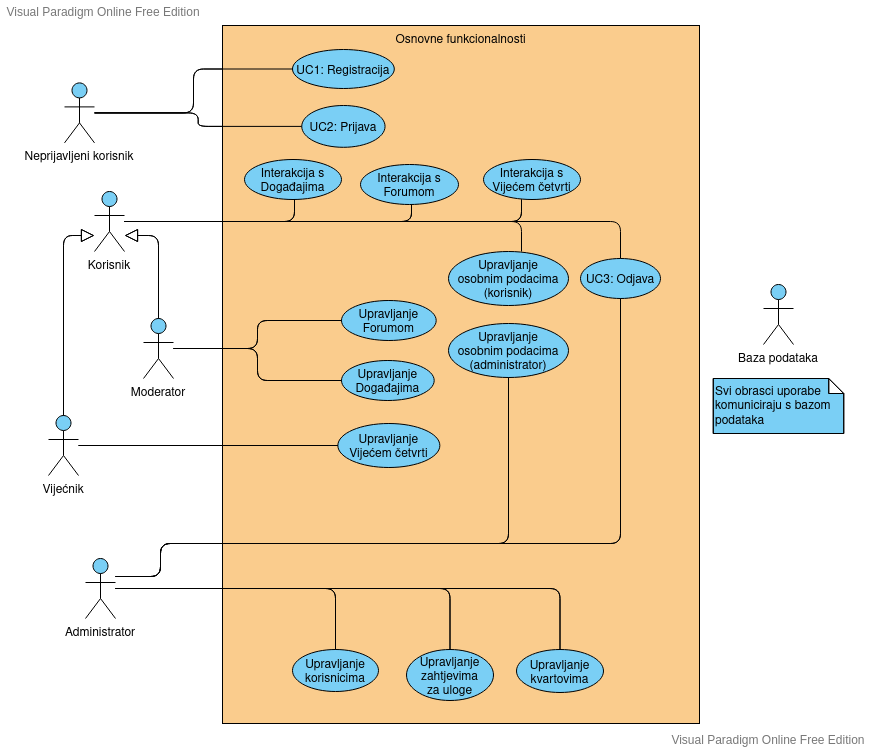
\includegraphics[width=\textwidth]{Dijagram_01.png}
					\caption{Dijagram obrazaca uporabe, osnovne funkcionalnosti}
					\end{figure}
					
					\item[] \begin{figure}[H]
					\centering
					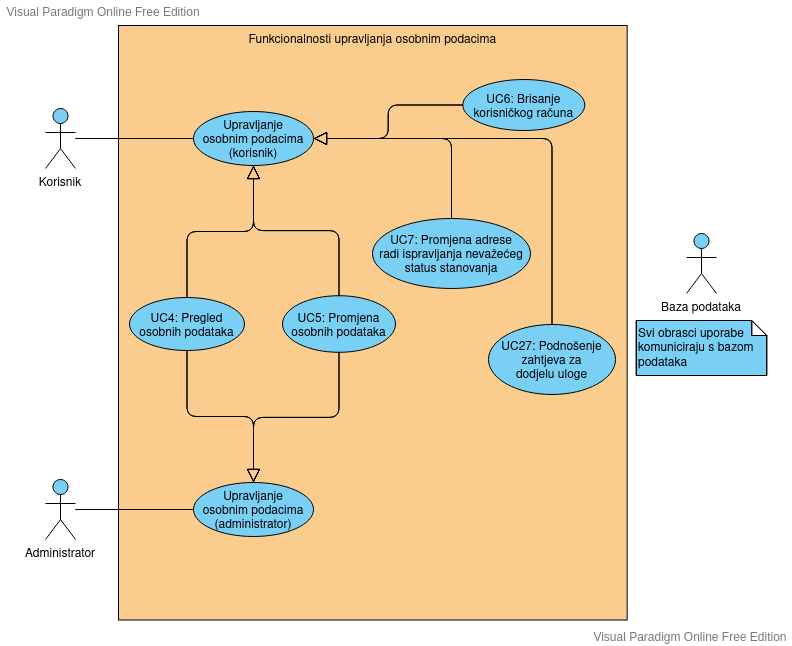
\includegraphics[width=\textwidth]{Dijagram_02.png}
					\caption{Dijagram obrazaca uporabe, funkcionalnosti upravljanja osobnim podacima}
					\end{figure}
					
					\begin{figure}[H]
					\centering
					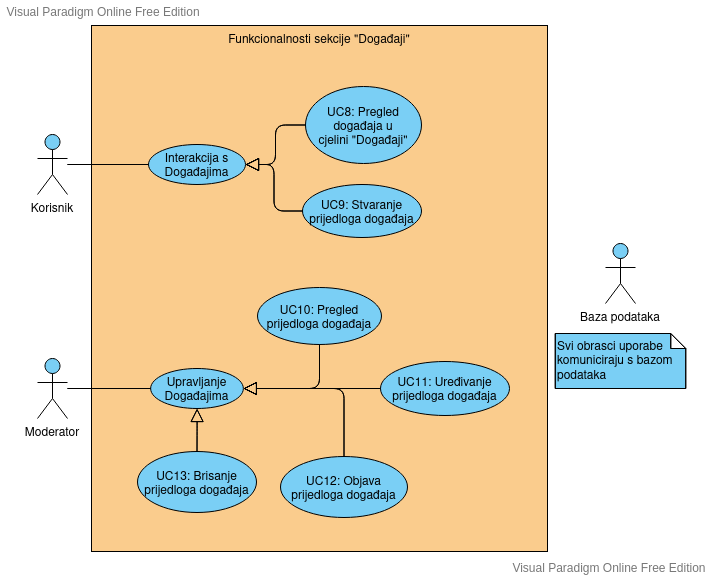
\includegraphics[width=\textwidth]{Dijagram_03.png}
					\caption{Dijagram obrazaca uporabe, funkcionalnosti sekcije događaji}
					\end{figure}
					
					\begin{figure}[H]
					\centering
					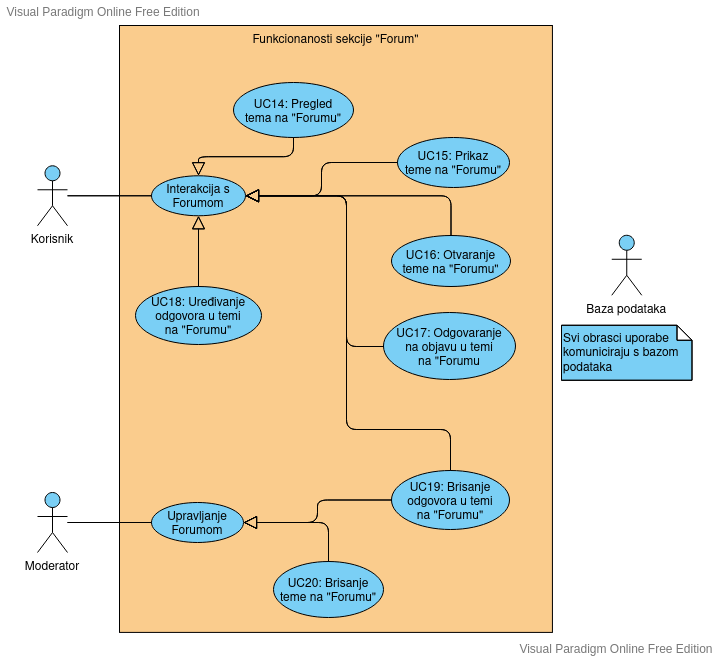
\includegraphics[width=\textwidth]{Dijagram_04.png}
					\caption{Dijagram obrazaca uporabe, funkcionalnosti sekcije "Forum"}
					\end{figure}
					
					\begin{figure}[H]
					\centering
					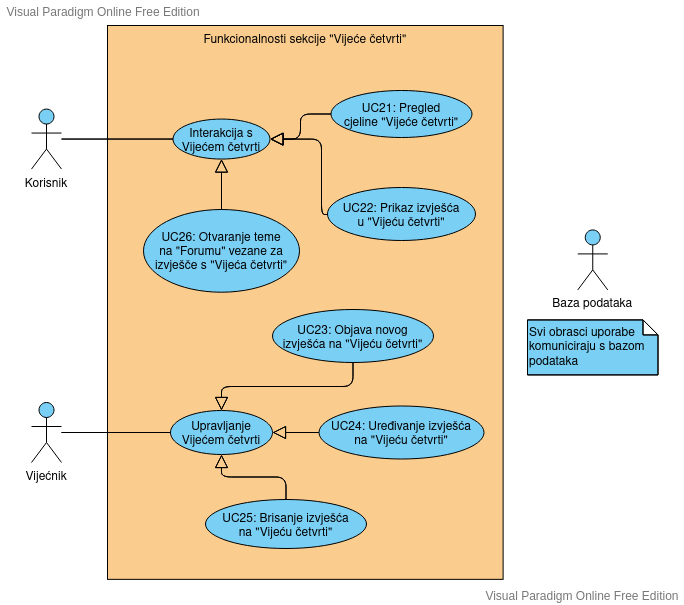
\includegraphics[width=\textwidth]{Dijagram_05.png}
					\caption{Dijagram obrazaca uporabe, funkcionalnosti sekcije "Vijeće četvrti"}
					\end{figure}
					
					\begin{figure}[H]
					\centering
					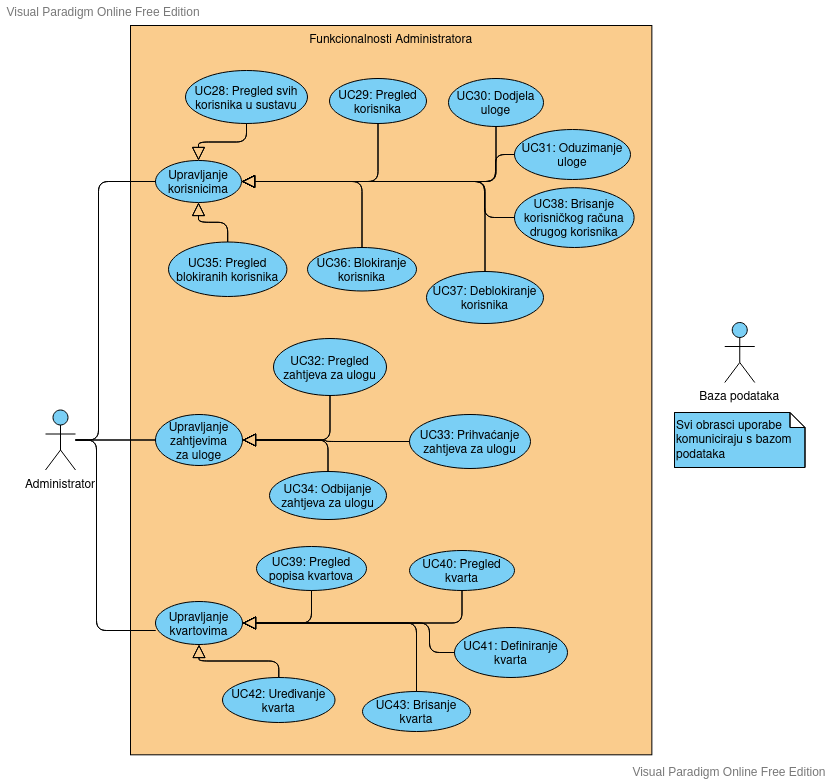
\includegraphics[width=\textwidth]{Dijagram_06.png}
					\caption{Dijagram obrazaca uporabe, funkcionalnosti Administratora}
					\end{figure}
				\end{packed_item}
				\eject	
				
			\subsection{Sekvencijski dijagrami}
		\noindent \textbf{Stvaranje, uređivanje, prihvaćanje i brisanje prijedloga događaja - obrasci uporabe UC9, UC10, UC11, UC12, UC13}
			
			
		\noindent Korisnik šalje zahtjev za stvaranjem prijedloga događaja. Poslužitelj prikazuje obrazac korisniku sa poljima naziv, mjesto, vrijeme, trajanje, kratak opis. Nakon što korisnik ispuni polja, poslužitelj traži potvrdu ispune prijedloga te korisnik potvrđuje spremanje prijedloga. Dok sva polja u obrascu nisu ispunjena poslužitelj upozorava korisnika. Ispunom praznih polja od strane korisnika, poslužitelj traži potvrdu promjene prijedloga te korisnik potvrđuje spremanje prijedloga poslužitelju. Baza podataka prima prijedlog od poslužitelja i pohranjuje promjene, vraća potvrdu izmjene poslužitelju, a poslužitelj potvrđuje spremanje prijedloga korisniku. Moderator započinje pregled prijedloga događaja, slanjem zahtjeva za prikaz prijedloga događaja poslužitelju.Poslužitelj dohvaća prijedloge događaja iz baze podataka te ih prikazuje moderatoru. Moderator odabire prijedlog događaja te poslužitelj prikazuje odabrani prijedlog. Dok sva polja nisu ispunjena poslužitelj upozorava moderatora da polja nisu ispunjena, moderator ispunjava prazna polja, poslužitelj traži potvrdu promjene te moderator sprema promjene. Ako prijedlog ne zadovoljava jezični standard, moderator mijenja polja, poslužitelj traži potvrdu promjene te moderator šalje zahtjev za spremanjem promjena poslužitelju. Poslužitelj nakon provedenih provjera i izmjena pohranjuje promjene na bazi podataka i vraća potvrdu spremanja moderatoru. Moderator šalje zahtjev za objavu prijedloga, poslužitelj pohranjuje promjene na bazi podataka i vraća potvrdu objave. Ukoliko Moderator šalje zahtjev za brisanje prijedloga, poslužitelj pohranjuje promjene na bazi podataka i vraća potvrdu
brisanja.  		
				\begin{figure}[H]
					\centering
					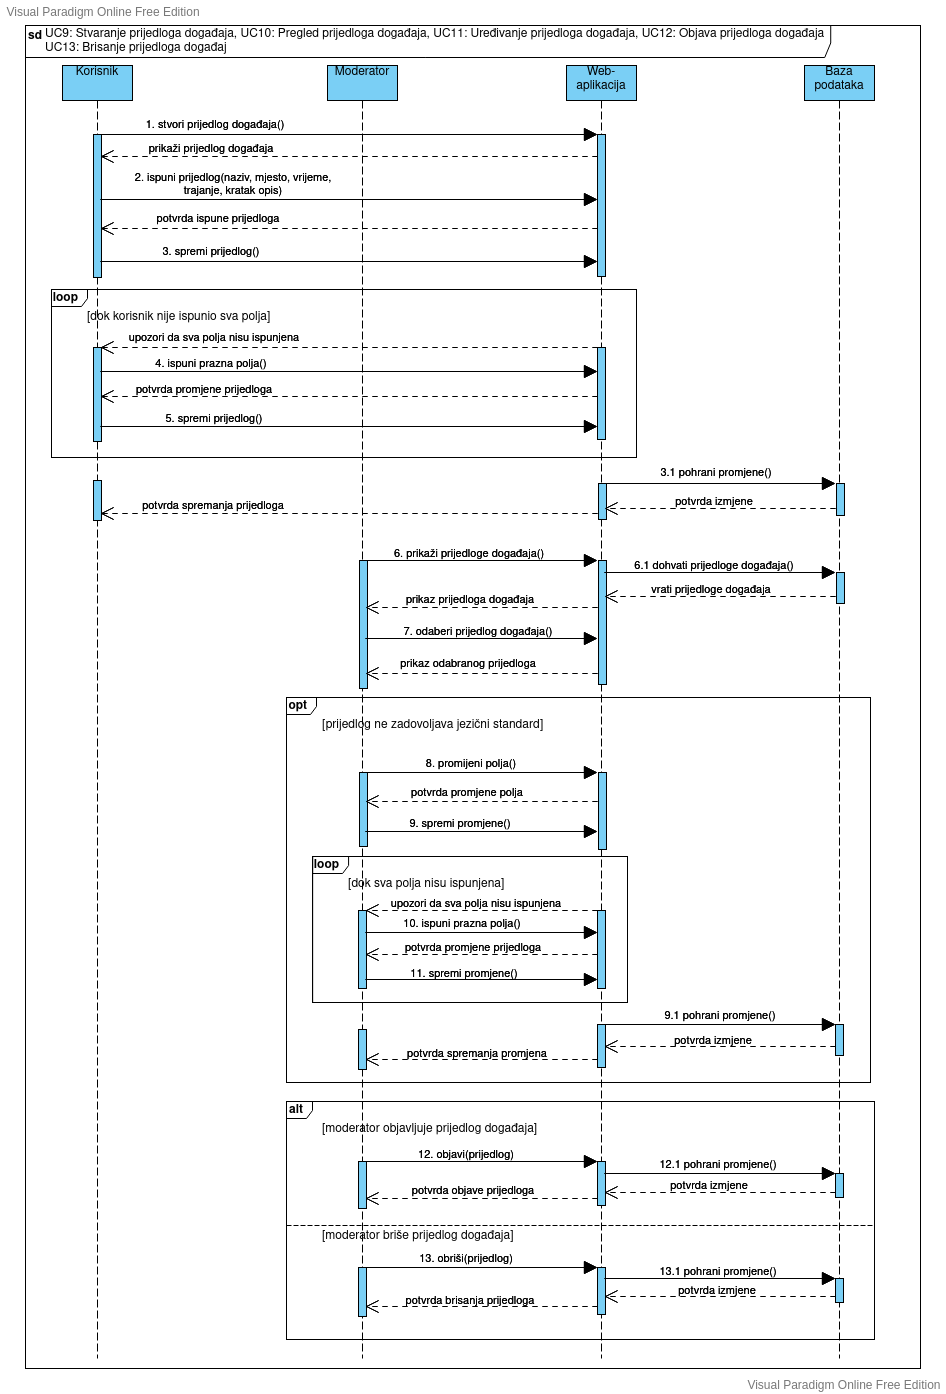
\includegraphics[width=\textwidth,keepaspectratio]{Dijagram_07.png}
					\caption{Sekvencijski dijagram za UC9, UC10, UC11, UC12, UC13}
				\end{figure}	
				\newpage			
		\noindent \textbf{Stvaranje, prihvaćanje i odbijanje zahtjeva za dodjelu uloge - obrasci uporabe UC27, UC32, UC33, UC34}
			
			
		\noindent Korisnik šalje poslužitelju zahtjev za stvaranje uloge, poslužitelj vraća 						prikaz zahtjeva. Nakon ispune zahtjeva poslužitelj traži potvrdu ispune zahtjeva 					te korisnik šalje zahtjev za dodjelu uloge. Poslužitelj pohranjuje 
				promjene na bazi podataka i nakon što baza potvrdi izmjene, 
				šalje potvrdu slanja zahtjeva korisniku. Administrator
				šalje zahtjev za prikaz zahtjeva za uloge. 
				Poslužitelj dohvaća zahtjeve iz baze podataka te ih prikazuje 
				administratoru. Administrator odabire željeni zahtjev te ga poslužitelj 							prikazuje. Administrator prihvaća odabrani
				zahtjev, poslužitelj pohranjuje promjene na bazi podataka i vraća potvrdu 						prihvata administratoru. Ukoliko 
				administrator odbije zahtjev, poslužitelj pohranjuje promjene 
				na bazi podataka te vraća potvrdu odbijanja 
				zahtjeva administratoru.
 
						
				\begin{figure}[H]
					\centering
					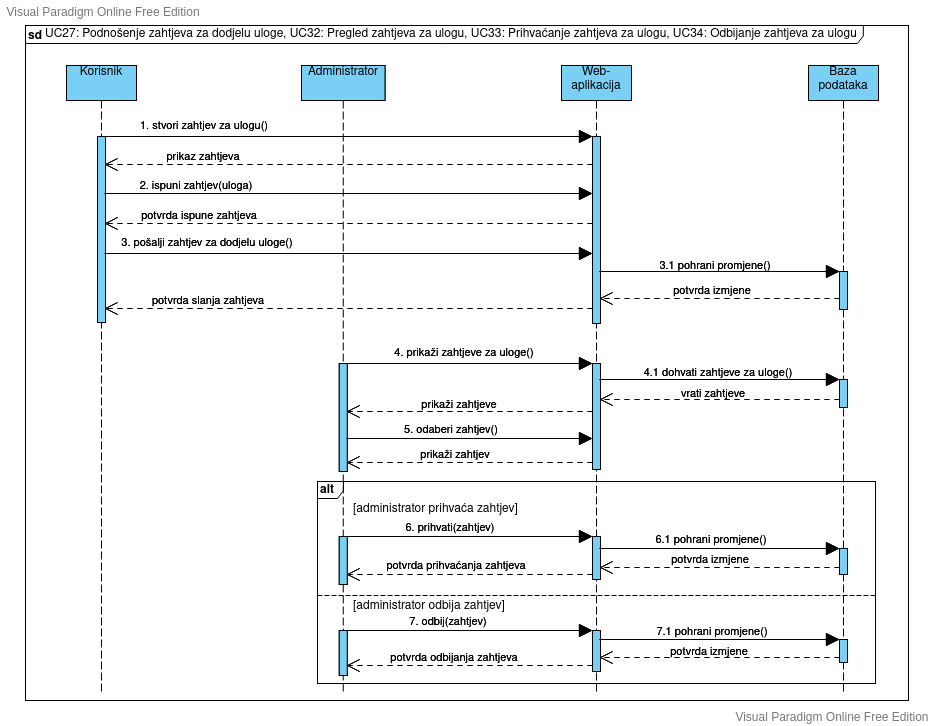
\includegraphics[width=\textwidth,keepaspectratio]{Dijagram_08.png}
					\caption{Sekvencijski dijagram za UC27, UC32, UC33, UC34}
				\end{figure}		
				\newpage		
		
		\noindent \textbf{Dodjela uloge - obrazac uporabe UC30}
			
			
		\noindent Administrator odabire željenu ulogu, poslužitelj vraća prikaz uloge te 							  administrator šalje zahtjev za dodijelu 
				  uloge. Poslužitelj provjerava postojanje zahtjeva jednakoj dodijeljenoj 
				  ulozi u bazi podataka. Ako zahtjev postoji
				  baza podataka vraća traženi zahtjev, poslužitelj mijenja status zahtjeva u 						  "prihvaćen" te baza podataka vraća
                   potvrdu izmjene. Ukoliko takav zahtjev ne postoji baza podataka vraća 								informaciju o nepostojanju traženog 
					zahtjeva. Poslužitelj vraća administratoru potvrdu izmjene.	
						
				\begin{figure}[H]
					\centering
					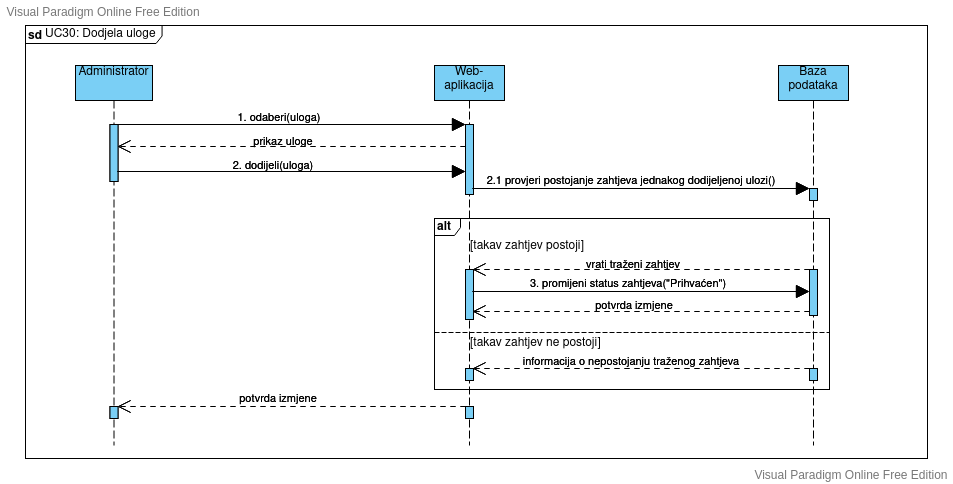
\includegraphics[width=\textwidth,keepaspectratio]{Dijagram_09.png}
					\caption{Sekvencijski dijagram za UC30}
				\end{figure}			
				\newpage	
		\noindent \textbf{Brisanje kvarta i promjena nevažećih adresa - obrasci uporabe UC43, UC7}
			
			
		\noindent Administrator šalje zahtjev poslužitelju za brisanjem kvarta. Poslužitelj 						odgovara sa upozorenjem o trajnosti 
				i nepovratnosti odabrane akcije. Ako administrator odabere odustati od brisanja 					kvarta, šalje zahtjev za
				odustajanjem poslužitelju te poslužitelj odgovara s potvrdom
 				odustajanja od brisanja kvarta. Ukoliko administrator
				odabere opciju potvrdi, šalje potvrdu za brisanjem poslužitelju. 
				Poslužitelj šalje zahtjev za brisanjem svih tema, događaja 
				i izvješća vezanih uz kvart na bazi podataka, baza vraća potvrdu izmjene te
 				poslužitelj šalje zahtjev za dohvat svih stanovnika obrisanog kvarta. 
 				Ako postoje takvi stanovnici, baza vraća
				tražene stanovnike, poslužitelj mijenja svim stanovnicima status stanovanja u 					neispravan, baza podataka šalje
				potvrdu izmjene poslužitelju. Ukoliko ne postoje takvi stanovnici, baza podataka 					šalje poslužitelju
 				informaciju o nepostojanju takvih stanovnika. Poslužitelj briše kvart, a baza 					podataka vraća potvrdu izmjene koju
				poslužitelj prosljeđuje do administratora. Korisnik koji ispravlja status 						nevažećeg statusa stanovanja
				 unosi novu adresu, poslužitelj šalje potvrdu te korisnik potvrđuje promjene. Dok 				unesena adresa nije validna
				poslužitelj upozorava korisnika da adresa nije valjana. Nakon što korisnik 						promijeni adresu, poslužitelj šalje
				potvrdu promjene adrese te korisnik sprema promjene. Poslužitelj pohranjuje 						promjene na bazi podataka, te nakon
				primitka potvrde izmjene, šalje potvrdu promjene adrese korisniku.
						
				\begin{figure}[H]
					\centering
					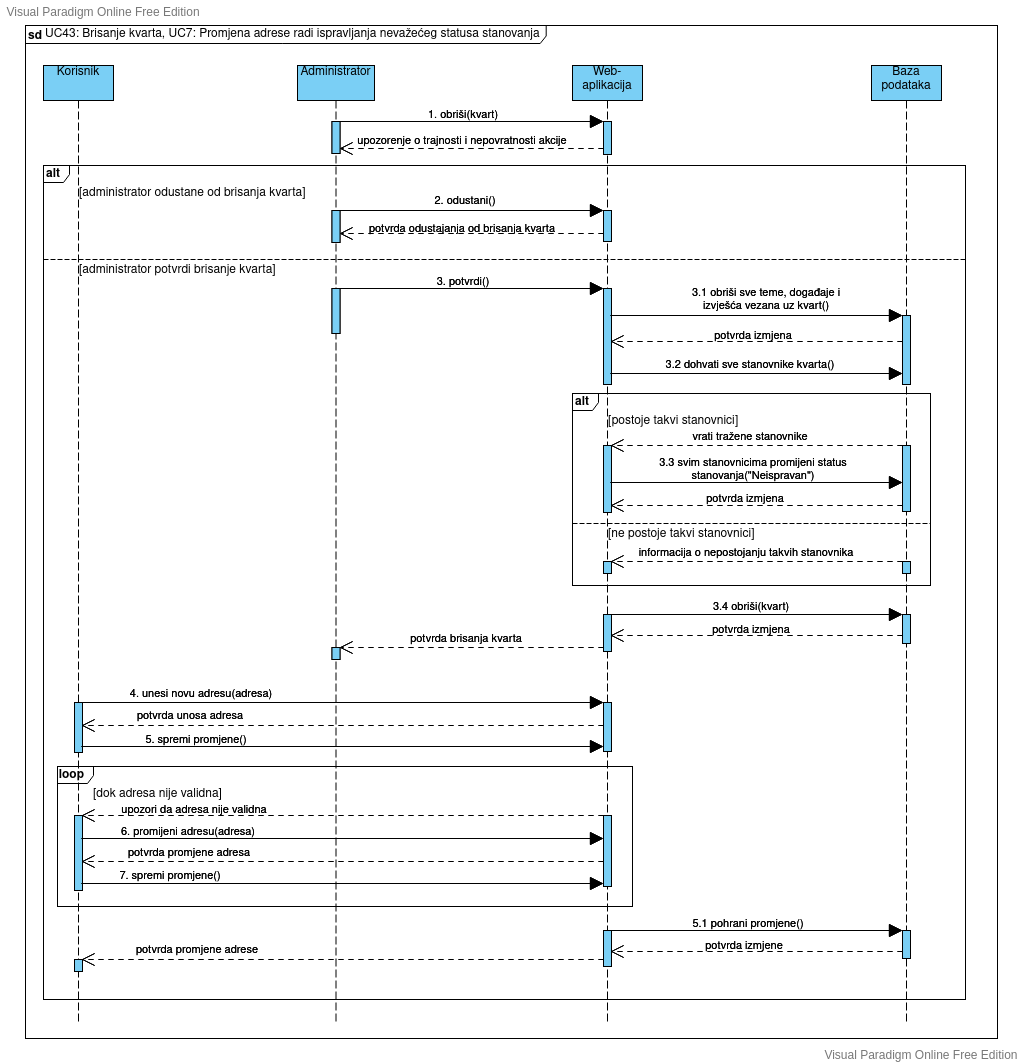
\includegraphics[width=\textwidth,keepaspectratio]{Dijagram_10.png}
					\caption{Sekvencijski dijagram za UC43, UC7}
				\end{figure}		
				
		
		
				\newpage
	
		\section{Ostali zahtjevi}
		\begin{packed_item}
						\item \textit{} Sustav treba koristiti hrvatski jezik te podržava hrvatsku abecedu
						\item \textit{} Sustav treba biti sposoban izvršavati sve zadatke u kratkom vremenu od najviše nekoliko sekundi
						\item \textit{} Sustav treba biti izrađen korištenjem objektno orijentirane paradigme u obliku web-aplikacije
						\item \textit{} Sustavu se pristupa iz javne mreže pomoću protokola HTTPS
						\item \textit{} Sustav omogućava istovremeni rad više korisnika
				
						\item \textit{} Korisnikovo neispravno korištenje ne smije poremetiti rad sustava
						\item \textit{} Sustav mora biti jednostavan za korištenje tako da ga je moguće koristiti bez uputa
						\item \textit{} Rad na sustavu ne smije narušavati funkcionalnosti sustava
						\item \textit{} Svi privatni podaci na sustavu su zaštićeni 
				
		\end{packed_item}
			 
			 
	